% `template.tex', a bare-bones example employing the AIAA class.
%
% For a more advanced example that makes use of several third-party
% LaTeX packages, see `advanced_example.tex', but please read the
% Known Problems section of the users manual first.
%
% Typical processing for PostScript (PS) output:
%
%  latex template
%  latex template   (repeat as needed to resolve references)
%
%  xdvi template    (onscreen draft display)
%  dvips template   (postscript)
%  gv template.ps   (onscreen display)
%  lpr template.ps  (hardcopy)
%
% With the above, only Encapsulated PostScript (EPS) images can be used.
%
% Typical processing for Portable Document Format (PDF) output:
%
%  pdflatex template
%  pdflatex template      (repeat as needed to resolve references)
%
%  acroread template.pdf  (onscreen display)
%
% If you have EPS figures, you will need to use the epstopdf script
% to convert them to PDF because PDF is a limmited subset of EPS.
% pdflatex accepts a variety of other image formats such as JPG, TIF,
% PNG, and so forth -- check the documentation for your version.
%
% If you do *not* specify suffixes when using the graphicx package's
% \includegraphics command, latex and pdflatex will automatically select
% the appropriate figure format from those available.  This allows you
% to produce PS and PDF output from the same LaTeX source file.
%
% To generate a large format (e.g., 11"x17") PostScript copy for editing
% purposes, use
%
%  dvips -x 1467 -O -0.65in,0.85in -t tabloid template
%
% For further details and support, read the Users Manual, aiaa.pdf.


% Try to reduce the number of latex support calls from people who
% don't read the included documentation.
%
\typeout{}\typeout{If latex fails to find aiaa-tc, read the README file!}
%


\documentclass[]{aiaa-tc}% insert '[draft]' option to show overfull boxes
\usepackage{amssymb, amsmath}
\usepackage{float}
 \title{Flight Testing Small UAVs for Aerodynamic Parameter Estimation}

 \author{
  Adam T. Chase%
    \thanks{Graduate Student, Aerospace Engineering, One Grand Avenue, AIAA Student Member.}\thanksibid{1}
  \ and Robert A. McDonald
\thanks{Associate Professor, Aerospace Engineering, One Grand Avenue, AIAA Senior Member.}\\
  {\normalsize\itshape
   California Polytechnic State University, San Luis Obispo, California 93407}\\
 }

 % Data used by 'handcarry' option if invoked
 \AIAApapernumber{YEAR-NUMBER}
 \AIAAconference{Conference Name, Date, and Location}
 \AIAAcopyright{\AIAAcopyrightD{YEAR}}

 % Define commands to assure consistent treatment throughout document
 \newcommand{\eqnref}[1]{(\ref{#1})}
 \newcommand{\class}[1]{\texttt{#1}}
 \newcommand{\package}[1]{\texttt{#1}}
 \newcommand{\file}[1]{\texttt{#1}}
 \newcommand{\BibTeX}{\textsc{Bib}\TeX}

\begin{document}

\maketitle

\begin{abstract}
This paper set out to measure in-flight aerodynamic force coefficients of small scale UAVs. A data acquisition system was developed that saves relevant state information to an attached SD card. This card can be offloaded at the test field, quickly processed, and aerodynamic parameter estimates of the vehicle are calculated. The system allows measurement of values critical to aircraft performance estimation, such as a drag polar, $C_L-\alpha$ curves, etc. This is can be done while the vehicle is in an unsteady flight condition, and can be applied to full-scale drag model validation of line-of-sight limited vehicles, as well as rapid and inexpensive testing during conceptual design. The data acquisition system was purposely designed to be upgradeable for future measurement needs.
\end{abstract}

\section*{Nomenclature}

\begin{tabbing}
  XXX \= \kill% this line sets tab stop
  $J$ \> Jacobian Matrix \\
  $f$ \> Residual value vector \\
  $x$ \> Variable value vector \\
  $F$ \> Force, N \\
  $m$ \> Mass, kg \\
  $\Delta x$ \> Variable displacement vector \\
  $\alpha$ \> Acceleration, m/s\textsuperscript{2} \\[5pt]
  \textit{Subscript}\\
  $i$ \> Variable number \\
 \end{tabbing}

\section{Introduction}
An accurate drag prediction is critical for conceptual aircraft design, aircraft mission planning, and predicting performance trends of comparable aircraft. To this end, industry spends an extensive amount of time and money developing wind tunnel models and executing wind tunnel tests. Additionally, it is difficult to impossible to exactly scale down a vehicle, especially when features such as rivets, servo control horns, antennas, and air data probes are included. These differences between the model and the as-built aircraft can cause accuracy of the wind tunnel test to suffer. This inaccuracy inevitably leads to aerodynamic flight tests that attempt to quantify the as-built drag and lift characteristics of the vehicle.

\indent
The flight test of full scale aircraft for drag polar prediction is often conducted about a trimmed condition, and is a method referred to as ``Cruise Testing"\cite{olson2000aircraft}. That is, the aircraft is flown to an operating conditions dictated by the test plan, and sets the control surfaces such that there are no accelerations and no moments. Data is then collected for a set amount of time, without changing the operating condition. After the data is collected, the operating point is changed, the aircraft is trimmed at this new flight condition, and data is again collected. This process is repeated at various points in the aircraft's flight envelope until enough data is collected to estimate a drag polar.

\indent
Unfortunately, for many R/C aircraft and small UAVs, this procedure isn't feasible. First, these aircraft typically operate close to ground level, meaning there could potentially be both unsteady and turbulent winds, and a steady wind. R/C aircraft and small UAVs typically have much lower moments of inertias, masses, and wing loadings than their full-scale counterparts, which means they will be affected much more by atmospheric disturbances than full-scale vehicles. Second, many of these aircraft have a line-of-sight communication link, and R/C aircraft in particular are flown in small patterns at a flight field. Even in the case of a steady atmosphere, R/C aircraft usually are not well trimmed, because by the time the pilot can see if the vehicle is trimmed, he has to turn around in the pattern. This paper attempts to fix these problems, by allowing the pilot to fly in a more generic flight path (unsteady flight condition), and not relying on a still atmosphere assumption.
\section{Previous Work}

There has been extensive work in this area, both in the estimation of small vehicle performance, and estimates of the individual required states. This section will review what has previously been accomplished.


\section{Method}
\label{background-information}
Some basic assumptions will apply throughout the modeling of dynamics in this paper. They are as follows:
\begin{enumerate}
\item The vehicle is a fixed mass.
\item Coriolis effects are negligible.
\item Thrust will be assumed to be 0.
\end{enumerate}
Note that a stationary atmosphere is not assumed.

For this paper, the reference frames used will follow those described in \cite{klein2006aircraft}.

\label{sys-desc}
Newton's 2nd Law of Motion states
\begin{align}
\vec{F} &= \frac{d}{dt}(m\vec{V})
\end{align}
where $\vec{F}$ is the sum of all applied forces, $\vec{m}$ is the mass of the vehicle, and $\vec{V}$ is the vehicle's velocity. Using the fixed mass assumption, this reduces to 
\begin{align}
\vec{F} &= m\frac{d\vec{v}}{dt}\\
&= m\vec{a}
\end{align}

The applied forces on the vehicle are 
\begin{align}
\vec{F} &= \vec{F}_{A}+\vec{F}_{G}+\vec{F}_{T}
\end{align}

where $\vec{F_{A}}$ accounts for all aerodynamic forces acting on the vehicle, $\vec{F_{G}}$ is the force due to gravity, and $\vec{F_{T}}$ accounts for forces from the propulsion system. Each of these forces will be discussed next.
Aerodynamic forces are described in the stability reference frame. In general, they are defined as

\begin{align}
\vec{F}_{A_S} &= D \hat{i}_s+Y \hat{j}_s+L \hat{k}_s
\end{align}

where $D$ is drag force, $Y$ is side force, and $L$ is lift force. 

The gravitational force on the vehicle acts in the $+z_{ned}$ direction and is equal in magnitude to the vehicle's weight $W$, leading to
\begin{align}
\vec{F}_{G_{ned}} &= 0\hat{i}_{ned}+0\hat{j}_{ned}+W\hat{k}_{ned}
\end{align}

In general, propulsive forces are modeled as
\begin{align}
\vec{F}_{T_b} &= T_x \hat{i}_b+T_y \hat{j}_b +T_z \hat{k}_b
\end{align}
where $T_x$, $T_y$, and $T_z$ are components of thrust in their respective body axis directions. However, as previously mentioned, propulsive forces are assumed to be $\vec{0}$ for this paper.

The forces are combined and transformed into the body axes reference frame so that they align with the output of body mounted accelerometers. The combined equations of motion are then

\begin{align}
\vec{F}_{AERO_W} = DCM_{bw}^{-1}(m\vec{a} - DCM_{ib}\vec{F}_{GRAVITY_i})
\end{align}


\subsection*{Kalman Filter Usage}
\label{kalman-filter}
This paper utilizes multiple Kalman Filters to estimate both regression coefficients and improved states. The Kalman filter operates recursively on a time-series and provides an optimal estimate of the system state.

\subsubsection*{Linear Kalman Filter}
A linear Kalman filter can be applied where the system in question can be described in the form \cite{welch1995introduction}

\begin{align}
x_k &= Ax_{k-1} + Bu_{k-1}+w_{k-1}
\end{align}
where $A$ is the state transition matrix, $x_{k-1}$ is the previous state, $B$ is the input matrix, $u_{k-1}$ is the input vector, and $w_{k-1}$ is random process noise.

The measured state is then 
\begin{align}
z_k &= Hx_k+v_k
\end{align} 

where $H$ is the output matrix and $v_k$ is measurement noise.

\indent
The Kalman filter operates in a predictor-corrector manner, where the predictor step is often called the \textit{a priori} estimate, and the corrector step is often called the \textit{a posteriori} estimate. The \textit{a priori} state estimate is calculated using prior states and inputs, while assuming no process noise

\begin{align}
\hat{x}^-_k &= A\hat{x}_{k-1}+Bu_{k-1}
\end{align}



The \textit{a priori} estimate of the covariance matrix is projected in a similar manner

\begin{align}
P^-_k &= AP_{k-1}A^T+Q
\end{align}

where Q the process noise covariance matrix.

The Kalman gain is calculated by combining the predicted, \textit{a priori} covariance matrix with the measurement noise covariance matrix $Q$

\begin{align}
K_k &=P^-_kH^T(HP^-_kH^T + R)^{-1}
\end{align}

This optimal Kalman gain is then used to estimate the \textit{a posteriori} estimate of the state and covariance matrix

\begin{align}
\label{kalmanStateUpdate}
\hat{x}_k &=\hat{x}^-_k+K_k(z_k-y_k)
\end{align}

\begin{align}
P_k &= (I-K_kH)P^-_k
\end{align}

where $y_k$ is the predicted value of $z_k$ found using the output matrix $H$ and the \textit{a priori} state estimate
\begin{align}
y_k &= H\hat{x}^-_k
\end{align}
Note that Equation \ref{kalmanStateUpdate} is essentially a weighted average of a measured state and an expected state. The weighting is the Kalman gain, which is related to the ratio of confidence in the measured state and the expected state. For a 1-D case with equal confidence between the measured state and the expected state, the Kalman gain $K_k = 0.5$, and the Kalman filter becomes a simple and straight-forward average.


\subsubsection*{Extended Kalman Filter}
\label{EKFTheory}
The Extended Kalman filter is used for a non-linear system and is essentially a linearization of a nonlinear plant. A non-linear system can be described as \cite{welch1995introduction}

\begin{align}
x_k &= f(x_{k-1},u_{k-1},w_{k-1})\\
z_k &= h(x_k,v_k)
\end{align}

The process noise $w_{k-1}$ and measurement noise $v_k$ are not known (or the Kalman filter would not be necessary), so the states are approximated assuming both noise sources are 0

\begin{align}
\tilde{x}_k &= f(\hat{x}_{k-1},u_{k-1},0)\\
\tilde{z}_k &= h(\tilde{x}_k,0)
\end{align}

The actual states are related to the approximate states by

\begin{align}
x_k &\approx\tilde{x}_k+A(x_k-\hat{x}_{k-1})+Ww_{k-1}\\
z_k &\approx\tilde{z}_k+H(x_k-\tilde{x}_{k-1})+Vv_k
\end{align}

where  the matrices $A$, $W$, $H$, and $V$ represent the different Jacobians matrices:
\begin{align}
A &= \frac{\partial f_i}{\partial x_j}(\hat{x}_{k-1},u_{k-1},0)\\
W &= \frac{\partial f_i}{\partial w_j}(\hat{x}_{k-1},u_{k-1},0)\\
H &= \frac{\partial h_i}{\partial x_j}(\hat{x}_{k},0)\\
V &= \frac{\partial h_i}{\partial v_j}(\hat{x}_{k},0)
\end{align}

The Extended Kalman Filter uses these linearized equations to perform the same process as the linear Kalman Filter. Again, the first step is to calculate the \textit{a priori} estimate of the state and the covariance matrix
\begin{align}
\hat{x}^-_k &=f(\hat{x}_{k-1},u_{k-1},0)\\
P^-_k  &= A_kP_{k-1}A^T_{k-1}+W_kQ_{k-1}W^T_k
\end{align}

Next, the Kalman gain is calculated
\begin{align}
K_k &=P^-_kH^T_k(H_kP^-_kH^T_k+V_kR_kV^T_k)^{-1}
\end{align}

The Kalman gain is then used to calculate the \textit{a posteriori} estimate of the state and covariance matrix

\begin{align}
\hat{x}_k &=\hat{x}^-_{k}+K_k(z_k-y_k)\\
\label{kalmanVariance}
P_k &=(I-K_kH_k)P^-_k
\end{align}

where $y_k$ is, as in the linear case, the predicted value of $z_k$, but calculated using the nonlinear output function and the \textit{a priori} state estimate

\begin{align}
y_k &= h(\hat{x}^-_k,0)
\end{align}

Unlike the linear Kalman filter, the Extended Kalman filter is not proven to be optimal. However, it has been utilized for a wide range of applications with excellent results.
\section{Simulation}
\label{simulation}
A 6-DOF flight simulator was used to validate the drag prediction method before hardware was purchased. The main utility of the simulator was to provide simulated flight test data with signals that contained no noise. The actual sensors during a flight test will be noisy signals, and Guassian white noise was added to the clean signals from the simulator to check the method's sensitivity to sensor noise. The flight simulator used was a model of the de Haviland Beaver (DHC-2)that comes as a demo in the Aerospace Toolbox of Simulink. 
 
\begin{figure}[h]
  \caption{Simulink's de Haviland Beaver Simulator} \label{dhc2Picture}
  \centering
    \includegraphics[width=0.5\textwidth]{figures/dhc2.png}
\end{figure}
The Simulink model was modified to output required signals to the workspace, which essentially created a sensor with zero noise. The mass, moments of inertia, and reference lengths were then scaled to those of a Zagi R/C aircraft found in \cite{stevens2003aircraft}. The original Simulink model was already connected to a FlightGear visualization engine, but the model was altered such that the indicators would function properly.
\begin{figure}[h!]
  \caption{FlightGear Integrated with DHC-2 Simulink Model} \label{flightgearPicture}
  \centering
    \includegraphics[width=0.4\textwidth]{figures/flightgear.png}
\end{figure}
The engine forces and moments were set to zero in the simulator, to match the assumption of a folding propeller.
The force calculations built into the Beaver Simulink model were replaced with a parabolic drag polar of the form

\begin{align}
C_D &= C_{D_0} + K*(C_L(\alpha)-C_{L_{min}})
\end{align}

The lift coefficient $C_L(\alpha)$ was nonlinear aerodynamic data from a NACA 0012 taken from \cite{osborne2007transitions}. While this approximation to a nonlinear drag polar does not capture the drag rise due to stall, it does represent the limited lifting capability of a real wing, making it more realistic than assuming the wing does not stall.
\subsection*{Simulation Results}
The most first result of the simulation testing was a verification of the correct equations of motion. The simulation was initialized with various initial states to ensure there was no dependence on initial conditions. The vehicle was then flown by an R/C aircraft pilot using a joystick attached the to simulation. It was noted early in the simulation testing that flying a sweep of speeds was beneficial, as a wider range of the drag polar was flown. This result was included in much of the flight test planning.
One of the main goals of the simulation was to verify the data analysis routines developed in Matlab did in fact match inputs to outputs. To do this, the simulation was flown and, when finished, no noise was added to the data. The results are shown in Figure \ref{dragPolarNoNoise}.

\begin{figure}[h!]
  \caption{Equations of Motion Verification (No Noise)} \label{dragPolarNoNoise}
  \centering
    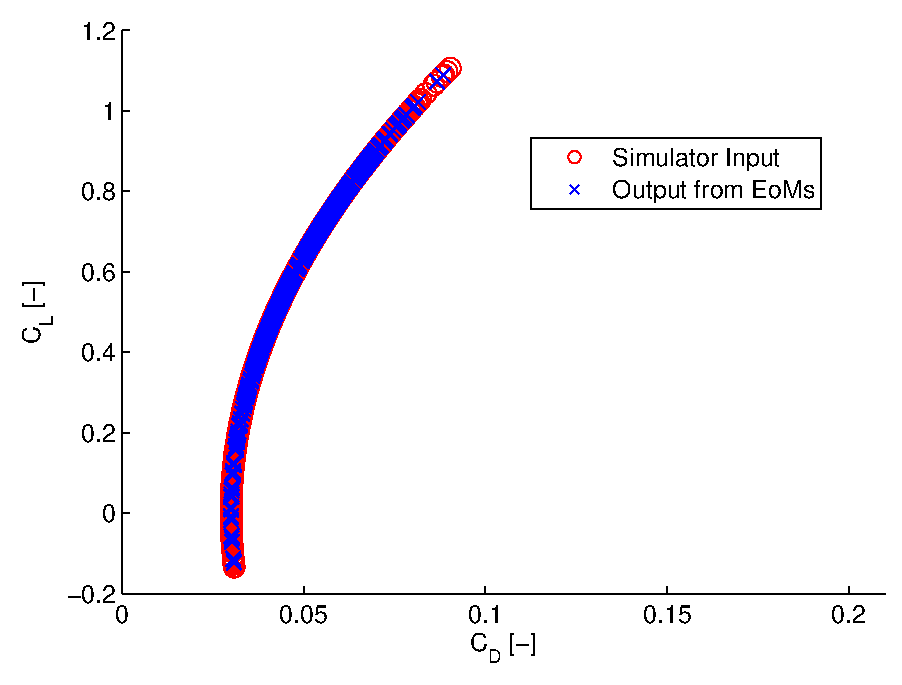
\includegraphics[width=0.5\textwidth]{figures/dragPolarNoNoise.eps}
\end{figure}

Figure \ref{dragPolarNoNoise} shows that the equations of motion used in the data analysis functions properly calculate the coefficients being passed into the system. With this result, noise was added to the system to see how sensitive coefficient estimation was to noise in each sensor. This process was a balancing act between available sensor accuracy and accuracy of the final solution. The final result guided sensor selection to those discussed in Section \ref{hardware}. To check if the final sensors chosen were acceptable, Gaussian noise was added to each state, with a mean of $0$ and a standard deviation equal to the root-mean-squared error listed in the manufacturer's data sheet for each sensor.
\begin{figure}[H]
  \caption{Drag Polar Prediction of Simulated Test Flight} \label{dragPolarNoise}
  \centering
    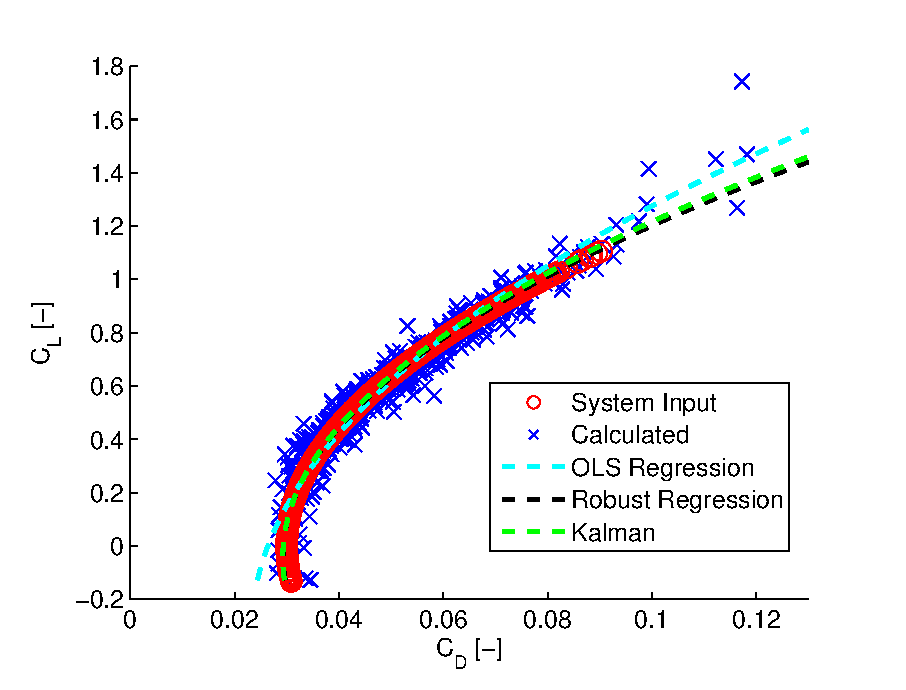
\includegraphics[width=0.5\textwidth]{figures/simDragPolarNoise.eps}
\end{figure}

For the particular simulated test flight shown in Figure \ref{dragPolarNoise}, the estimated drag polar coefficients had error coefficients outlined in Table \ref{simCoeffErrorTable}.

\begin{table}[H]
\caption{Nonlinear Model Results} % title of Table
\centering % used for centering table
\begin{tabular}{c c c c} % centered columns (4 columns)
\hline\hline %inserts double horizontal lines
 & $C_{D_0}$ & $K_1$ & $K_2$ \\ [0.5ex] % inserts table 
%heading
\hline % inserts single horizontal line
System Inputs & 0.0493 & 0 & 0.03 \\ % inserting body of the table
OLS Estimate & 0.0516 & -0.0056 & 0.0317 \\
Robust LS Estimate & 0.0500 & -0.0035 & 0.0313 \\ [1ex] % [1ex] adds vertical space
\hline %inserts single line
\end{tabular}
\label{simCoeffErrorTable} % is used to refer this table in the text
\end{table}

The results of this simulated flight test showed that the measurement system outlined in Section \ref{hardware} predicted the simulated drag polar with a reasonable error.

\section{Hardware}
\label{hardware}
Hardware selection was approached from a ``minimum sensor" perspective. One of the main goals of this paper was to reduce the number of sensors as much as possible to increase the variety of planes the hardware can fly on. To accomplish this, sensors were separated based on which state they could estimate.
\subsection*{Accelerations}
The accelerometer chosen for this paper was the ADXL-362 from Analog Devices. It has a noise error of $175\mu\text{g}/\sqrt{\text{Hz}}$ and has a 3.3V digital SPI interface\cite{adxl362DataSheet}. The accelerometer was purchased on a breakout board sold from Sparkfun Electronics.
\subsection*{Vehicle Mass}
All test vehicles will be weighed using a U-Line H-1650 counting scale. The scale has an accuracy of 0.001 lbs and a maximum capacity of 30 lbs. The minimum capacity of the scale is 10 grams \cite{U-Line}.
\subsection*{Euler Angles}
The Euler angles of the aircraft can be estimated using either an 3-d electronic compass or a 3-d mangetometer. A magnetometer reads the direction and magnitude of a magnetic field, while a compass combines a magnetometer with accelerometer readings to produce a more accurate estimate of the true angles. A Honeywell HMR-3500 3-d electronic compass was used for this paper. This compass provides a standard deviation of repeatability in roll of $0.2^\circ$ and a standard deviation of repeatabiltiy in pitch of $0.1^\circ$. Additionally, the heading accuracy is typically a standard deviation of $0.5^\circ$ \cite{honeywellHMR3500}. 

For increased accuracy, a discrete linear Kalman filter is applied. This necessitated adding a three-axis gyroscope to the system. The gyroscope chosen was the Invensense ITG-3200. This gyroscope has a total error of $0.38^\circ/$s-rms, and uses a digital I$^2$C interface that can have its logic level voltage defined on an input pin. The gyroscope has a selectable full-scale span that goes up to $\pm2000^\circ/$s. The gyroscope was purchased in breakout board form from Sparkfun Electronics \cite{itg3200DataSheet}.
With the angular rates available from the gyroscope, the system equations for the Kalman filter are
\begin{align}
\begin{bmatrix}
\phi_{k}\\
\theta_{k}\\
\psi_{k}
\end{bmatrix} & = \begin{bmatrix}
1 & 0 & 0\\0 & 1 & 0\\0 & 0 & 1
\end{bmatrix}\begin{bmatrix}
\phi_{k-1}\\
\theta_{k-1}\\
\psi_{k-1}
\end{bmatrix}
+ \begin{bmatrix}
\Delta T & 0 & 0 \\ 0 & \Delta T & 0\\0 & 0 & \Delta T
\end{bmatrix}\begin{bmatrix} 
p_k \\ q_k \\ r_k 
\end{bmatrix}+\hat{w}_{k-1}\\
z_k & = \begin{bmatrix}
1 & 0 &0\\0&1&0\\0&0&1
\end{bmatrix}\begin{bmatrix}
\phi_{k}\\
\theta_{k}\\
\psi_{k}
\end{bmatrix}+\hat{v}_{k-1}
\end{align}

The measurement covariance noise matrix was calculated using the standard deviation of the calibration data for the magnetometer, and the process noise covariance matrix was calculated using the standard deviation of the calibration data for the rate gyroscope.
\subsection*{Wind Angles}
The accuracy at which the aerodynamic wind angles are calculated is critical to the overall prediction accuracy. In keeping with the goal of minimizing the number of required sensors, an attempt was made to estimate aerodynamic angles without directly measuring them. There has been a plethora of work conducted on this subject. One of the first available papers on the subject was from the Air Force Institute of Technology \cite{joseph1988}. In that paper, two methods were developed: one for in flight estimation, and the other for post-flight estimation. Both methods relied on either estimated or known stability derivatives. Since the purpose of this paper is to estimate part of the dynamics, this estimating scheme will not work. Other techniques assume linearization about an operating condition \cite{morelli2012real}. For R/C aircraft this assumption generally cannot be made due to visual flight rules. Other work \cite{Lie2013} combined a dynamics model and a no-vertical-wind assumption. The overarching theme of this previous estimation work was that too many assumptions needed to be made to get results that were not accurate enough ($\approx1^\circ-2^\circ$) for drag polar estimation. For this reason, it was necessary to directly measure airflow angles.

A five-hole probe was chosen to measure aerodynamic angles as they do not contain moving parts and can provide very accurate, repeatable data. The five-hole probe selected was the Aeroprobe Air Data probe. It has a length of 6 inches and a diameter of 1/8 inch and has an integrated thermocouple for temperature measurement. Each line of the air data probe is connected to a Honeywell Integrated Pressure Transducer (IPT), model number IPT0001D33R. These are 1 PSI differential pressure sensors with a total error band of 0.2\% of full scale. They have a digital SPI interface that operates on a 3.3V logic level and output both a 24-bit pressure and a 16-bit temperature readings \cite{HoneywellIPTDataSheet}.

\indent

To improve the accuracy of the wind angle estimation, a discrete, an Extended Kalman filter was used. The state transition functions are nonlinear and are
\begin{align}
\dot{\alpha} & = \frac{1}{V\cos\beta}(-a_x\sin\alpha+a_z\cos\alpha)+q-(p\cos\alpha+r\sin\alpha)\tan\beta\\
\dot{\beta} &=\frac{1}{V}(-a_x\cos\alpha\sin\beta+a_y\cos\beta-a_z\sin\alpha\sin\beta)+p\sin\alpha-r\cos\alpha
\end{align}

The equations for the Kalman filter for the wind angles are
\begin{align}
\begin{bmatrix}
\alpha_k\\\beta_k
\end{bmatrix} &= \begin{bmatrix}
1& 0\\0&1
\end{bmatrix}\begin{bmatrix}
\alpha_{k-1}\\\beta_{k-1}
\end{bmatrix}+\begin{bmatrix}
\Delta T& 0\\0&\Delta T
\end{bmatrix}\begin{bmatrix}
\dot{\alpha_{k}}\\\dot{\beta_{k}}
\end{bmatrix}+\hat{w}_{k-1}\\
z_k & = \begin{bmatrix}
1 & 0\\0&1
\end{bmatrix}\begin{bmatrix}
\alpha_{k}\\
\beta_{k}
\end{bmatrix}+\hat{v}_{k-1}
\end{align}

The process covariance matrix was calculated using the error propogation discussed in Section \ref{pointErrorSection} and the standard deviation data from calibration of each of the sensors. The measurement noise covariance matrix was calculated based on the standard deviation data for the 5-hole probe calibration.

\subsection*{Flight Computer}
The flight computer chosen was an Arduino Due. This board has a 32-bit ARM processor, 54 digital I/O pins, 12 analog input pins, and 2 analog output pins. 
One of the main differences between this board and other Arduinos is that the Due operates on a 3.3V logic level instead of the normal 5V. This means sensors such as the HMR-3500 compass need logic level converters. To this end, logic level converters were purchased from Sparkfun. They are 2 channel, bi-directional converters and come in breakout board form. While the Arduino Due operates a 3.3V digital I/O system, it does provide a 5V source. This source powers the higher voltage side of the logic-level converter

\subsection*{Additional Sensors}
A uBlox LEA-6T GPS receiver was included in the data acquisition system to aid in mission visualization. This model was selected for its ability to output raw timing data, which can be used to get an extremely accurate inertial velocity estimate\cite{ubloxDemo}. The receiver itself was integrated onto a board sold by CGS Shop and has UART,USB, and I$^2$C interface options.

A barometric altitude sensor was also included the data acquisiton system. The model chosen was another Honeywell IPT, model number IPT0020A33. This sensor has reads absolute pressures to 20 PSI with a total error bound of 0.04\% of full scale. It communicates using a 3.3V SPI interface and outputs 24-bit pressure and 16-bit temperature readings.

\bibliographystyle{unsrt}
\bibliography{bibliography}

\end{document}

% - Release $Name:  $ -
